\newpage
\section{Countermeasure}
\begin{figure}[!ht]
\begin{center}
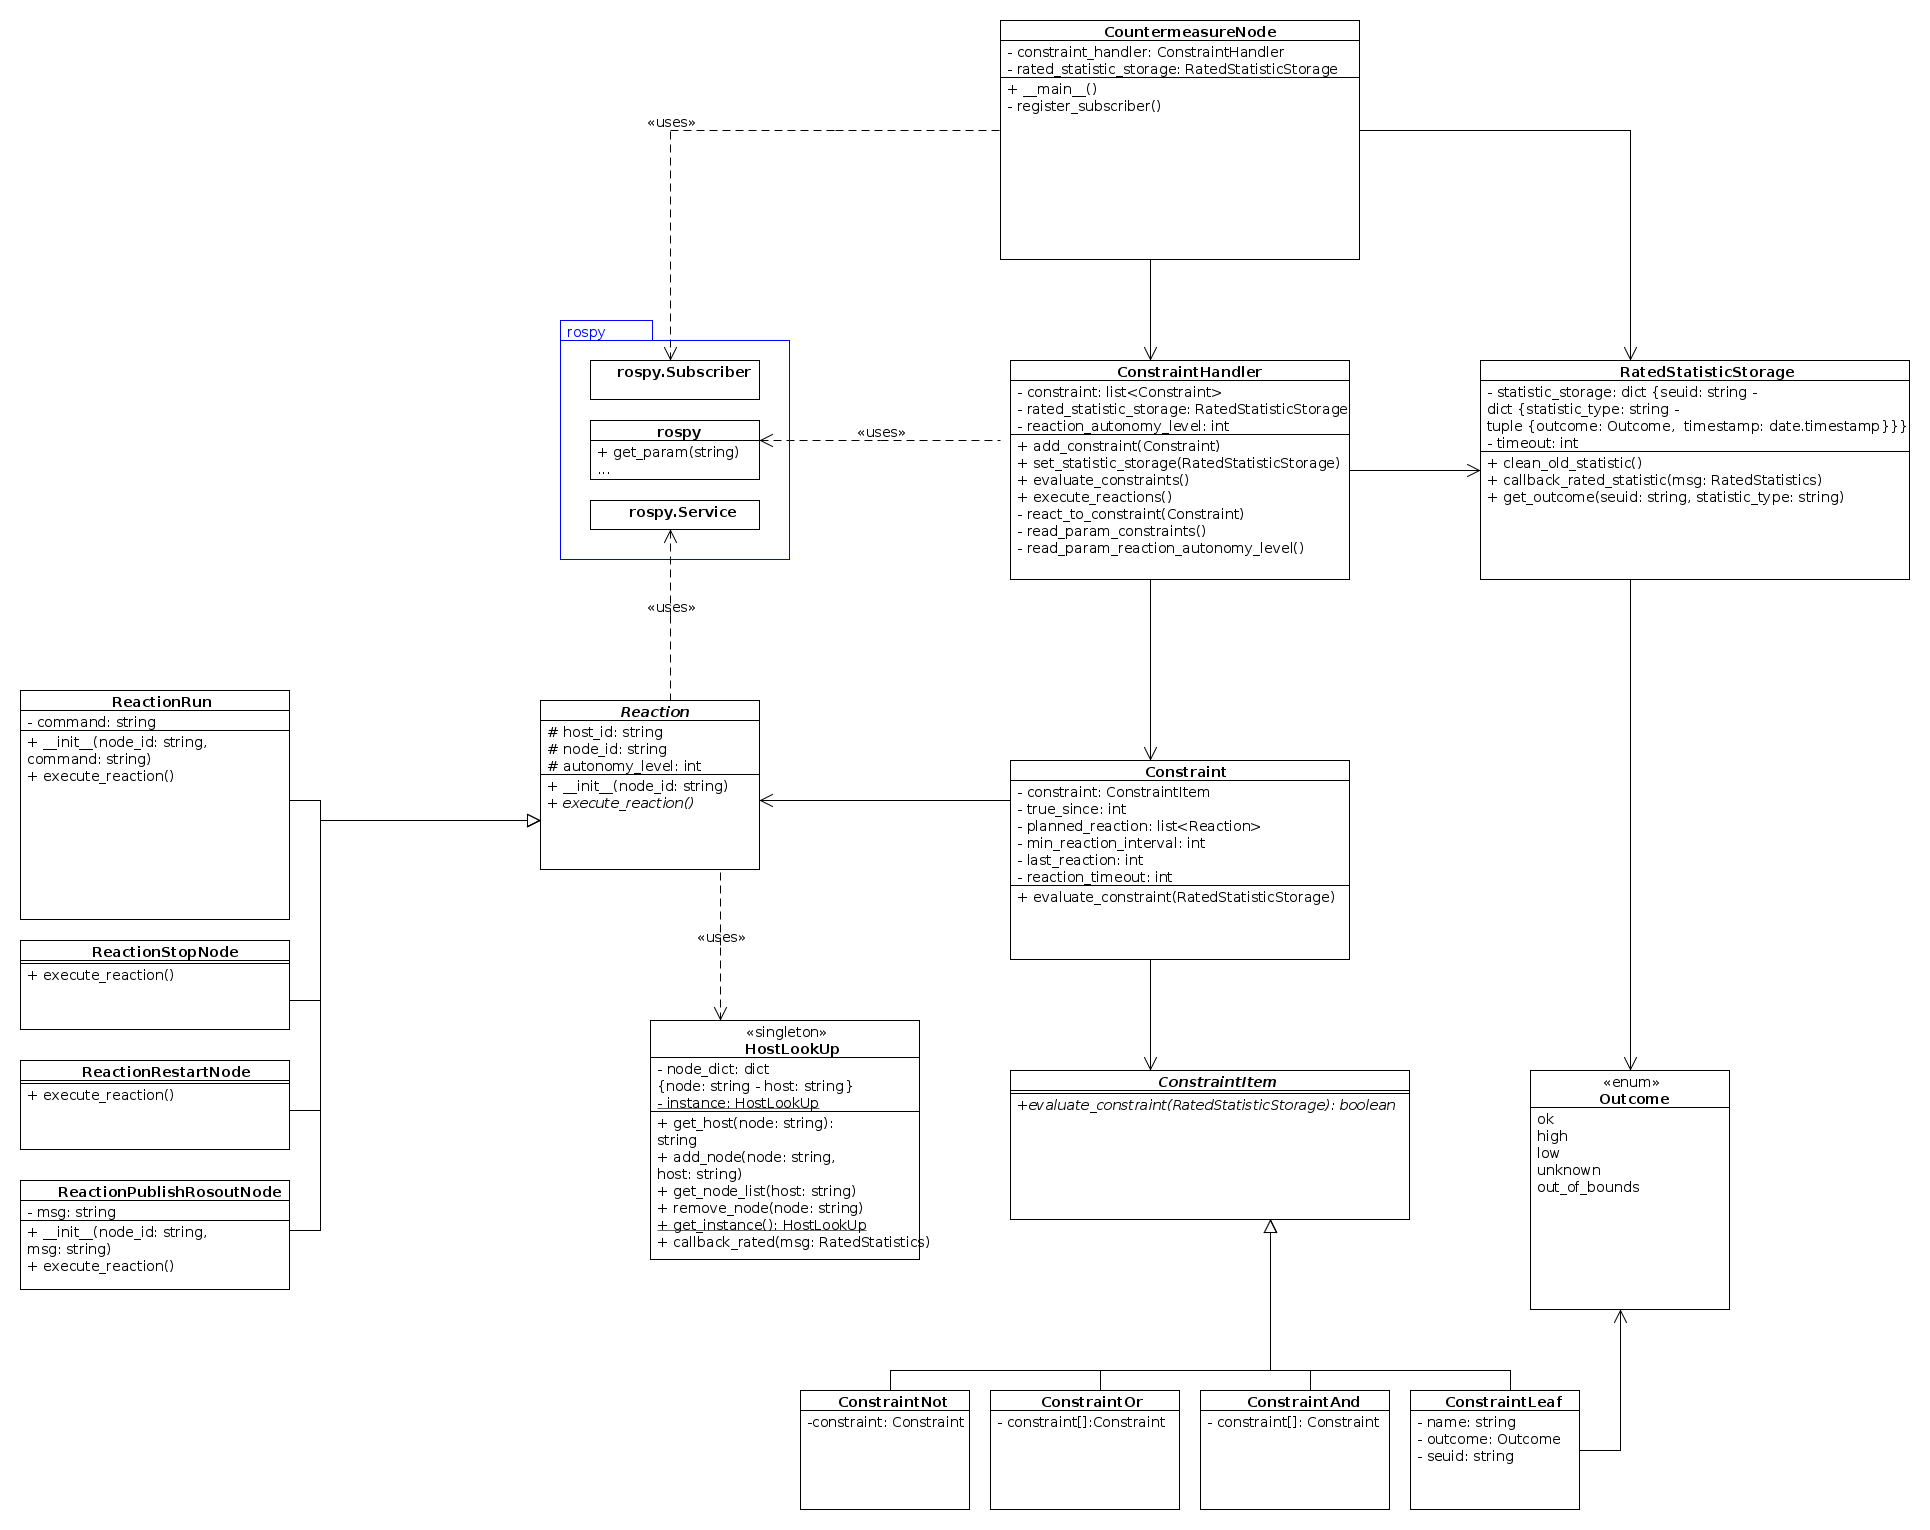
\includegraphics[width=1.0\linewidth]{./diagram_pictures/reactor/reactor.png}
\caption{The UML diagram of the countermeasure package}
\end{center}
\end{figure}

\mbox{}

\newpage


\newpage
\subsection{CountermeasureNode}
\begin{figure}[htbp]
	\begin{minipage}[t]{8cm}
		\vspace{0pt}
		\centering
		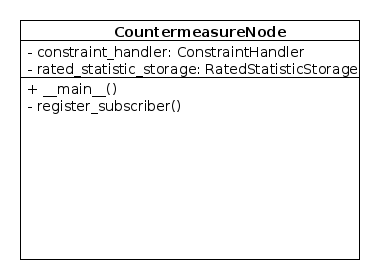
\includegraphics[scale=0.6]{./diagram_pictures/reactor/CountermeasureNode.png}
		\caption{The CountermeasureNode}
	\end{minipage}
	\hfill
	\begin{minipage}[t]{8cm}
		\vspace{10pt}
			A ROS node. Evaluates incoming rated statistics with a list of constraints. If those constraints turn out to be true appropriate action is taken.
	\end{minipage}
\end{figure}  


\subsubsection{Attributes}
\begin{itemize}
	\item \textbf{ private ConstraintHandler constraint\_handler}\\
		The handler for all constraints.
	\item \textbf{ private RatedStatisticStorage rated\_statistic\_storage}\\
		The storage of all incoming rated statistic.
\end{itemize}
\subsubsection{Methods}
\begin{itemize}
	\item \textbf{ public void \_\_main\_\_() }\\\\
		Periodically (threading) evaluates the constraints and cleans old statistics.
	\item \textbf{ private void register\_subscriber() }\\
		Registers to the rated statistics.
\end{itemize}


\newpage
\subsection{ConstraintHandler}
\begin{figure}[htbp]
	\begin{minipage}[t]{8cm}
		\vspace{0pt}
		\centering
		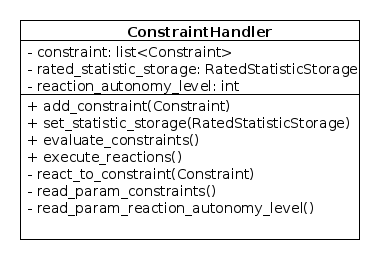
\includegraphics[scale=0.6]{./diagram_pictures/reactor/ConstraintHandler.png}
		\caption{The ConstraintHandler}
	\end{minipage}
	\hfill
	\begin{minipage}[t]{8cm}
		\vspace{10pt}
			Manages all constraints, checks if they are true and executes appropriate reactions if neccessary.
	\end{minipage}
\end{figure}  


\subsubsection{Attributes}
\begin{itemize}
	\item \textbf{ private list<Constraint> constraint\_list }\\
		Contains a list of all constraints.
	\item \textbf{ private  RatedStatisticStorage rated\_statistic\_storage }\\
		Contains all incoming rated statistic.
	\item \textbf{ private  int reaction\_autonomy\_level }\\
		Only reactions with an autonomy\_level <= reaction\_autonomy\_level get executed.
\end{itemize}
\subsubsection{Methods}
\begin{itemize}
	\item \textbf{ public void add\_constraint(Constraint)  }\\
		Adds an constraint to this list.
	\item \textbf{ public void set\_statistic(RatedStatisticStorage)  }\\
		Sets the Statistic to use. Should only be needed on initialisation.
	\item \textbf{ public void evaluate\_constraints()  }\\
		Evaluates every constraint.
	\item \textbf{ public void execute\_reactions()  }\\
		Checks if there are any new reactions to do and executes them.
	\item \textbf{ private void react\_to\_constraint(Constraint)  }\\
		Executes an single Reaction and updates the attributes of the Constraint.
	\item \textbf{ private void read\_param\_constraints()  }\\
		Reads all constraints from the parameter server.
	\item \textbf{ private void read\_param\_reaction\_autonomy\_level()  }\\
		Reads the reaction\_autonomy\_level from the parameter server.
\end{itemize}

\newpage
\subsection{RatedStatisticStorage}
\begin{figure}[htbp]
	\begin{minipage}[t]{10cm}
		\vspace{0pt}
		\centering
		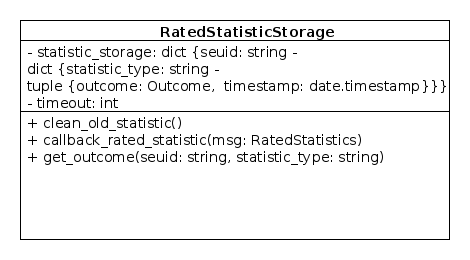
\includegraphics[scale=0.6]{./diagram_pictures/reactor/RatedStatisticStorage.png}
		\caption{The RatedStatisticStorage}
	\end{minipage}
	\hfill
	\begin{minipage}[t]{6cm}
		\vspace{10pt}
			A database which contains the current state of all rated statistics.
	\end{minipage}
\end{figure}  

\subsubsection{Attributes}
\begin{itemize}
	\item \textbf{ private dict\{string seuid - dict\{string statistic\_type - tuple\{Outcome outcome,date.timestamp timestamp\}\}\} statistic\_dict }\\
		A dictionary containing all rated statistic information with their outcome and an timestamp when they got added / updated to the dictionary.
	\item \textbf{ private int timeout }\\
		The timeout after which an item in ratedstatistic is declared too old and should be removed from the dict.
\end{itemize}
\subsubsection{Methods}
\begin{itemize}
	\item \textbf{ public void clean\_old\_statistic() }\\
		Checks the complete dictionary for statistics older than timeout seconds and removes them.
	\item \textbf{ public void callback\_rated\_statistic(RatedStatistics msg) }\\
		Callback for incoming rated statistics. Adds them to the dictionary or removes items from the dictionary if the rated statistic says that its within bounds again. 
	\item \textbf{ public Outcome get\_outcome(string seuid, string statistic\_type) }\\
		Returns the outcome of the specific seuid and statistic\_type.
\end{itemize}

\newpage
\subsection{Constraint}
\begin{figure}[htbp]
	\begin{minipage}[t]{8cm}
		\vspace{0pt}
		\centering
		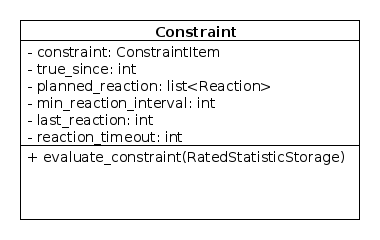
\includegraphics[scale=0.6]{./diagram_pictures/reactor/Constraint.png}
		\caption{The Constraint class}
	\end{minipage}
	\hfill
	\begin{minipage}[t]{8cm}
		\vspace{10pt}
			Contains the whole constraint with corresponding reactions
	\end{minipage}
\end{figure}  


\subsubsection{Attributes}
\begin{itemize}
	\item \textbf{ private ConstraintItem constraint }\\
	First constraint in the chain of ConstraintItems.
	\item \textbf{ private int true\_since }\\
	Epoch time in milliseconds since the constraint is true,
	if the constraint is not true it is 0.
	\item \textbf{ private list<Reaction> planned\_reaction }\\
	An list of reactions that should be executed if the constraint has been true longer than min\_reaction\_interval milliseconds.
	\item \textbf{ private int min\_reaction\_interval }\\
	The minimum time needed in ms that the constraint needs to be true to execute the planned\_reaction.
	\item \textbf{ private int last\_reaction }\\
	Contains the epoch time in ms when the reaction corresponding to this constraint has been executed for the last time.
		It is 0 if it has never been executed.
	\item \textbf{ private int reaction\_timeout }\\
	Minimum durotation in ms needed before an reaction can happen again.
\end{itemize}
\subsubsection{Methods}
\begin{itemize}
	\item \textbf{ public void evaluate\_constraint(RatedStatisticStorage)  }\\
	Evaluates this constraint and sets the attributes according to the result of the evaluation.
\end{itemize}



\newpage
\subsection{ConstraintItem}
\begin{figure}[htbp]
	\begin{minipage}[t]{8cm}
		\vspace{0pt}
		\centering
		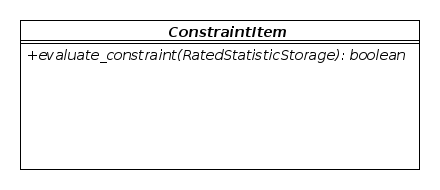
\includegraphics[scale=0.6]{./diagram_pictures/reactor/ConstraintItem.png}
		\caption{The ConstraintItem class}
	\end{minipage}
	\hfill
	\begin{minipage}[t]{6.5cm}
		\vspace{10pt}
			Abstract description of a Constraint, can be an logical operation on constraints or an actual constraint.
	\end{minipage}
\end{figure}  


\subsubsection{Attributes}
\subsubsection{Methods}
\begin{itemize}
	\item \textbf{ public abstract boolean evaluate\_constraint(RatedStatisticStorage) }\\
	Evaluates if this constraint, given the available RatedStatisticStorage, is true. 
\end{itemize}		


\newpage
\subsection{ConstraintLeaf}
\begin{figure}[htbp]
	\begin{minipage}[t]{8cm}
		\vspace{0pt}
		\centering
		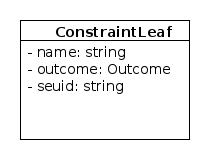
\includegraphics[scale=0.6]{./diagram_pictures/reactor/ConstraintLeaf.png}
		\caption{The ConstraintLeaf class}
	\end{minipage}
	\hfill
	\begin{minipage}[t]{8cm}
		\vspace{10pt}
			Contains an actual constraint.
	\end{minipage}
\end{figure}  

\subsubsection{Attributes}
\begin{itemize}
	\item \textbf{ private string name }\\
	Contains the name of the statistic data.
	\item \textbf{ private Outcome outcome }\\
	Contains the outcome needed for this constraint to be true.
	\item \textbf{ private string seuid }\\
	Contains the unique identifier of the corresponding StatisticEntity.
\end{itemize}
\subsubsection{Methods}
\begin{itemize}
	\item \textbf{ public abstract boolean evaluate\_constraint(RatedStatisticStorage) }\\
	Returns true if this constrain is true for the RatedStatisticStorage.
\end{itemize}


\newpage
\subsection{ConstraintAnd}
\begin{figure}[htbp]
	\begin{minipage}[t]{8cm}
		\vspace{0pt}
		\centering
		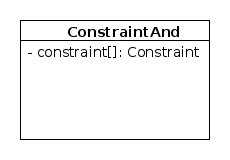
\includegraphics[scale=0.6]{./diagram_pictures/reactor/ConstraintAnd.png}
		\caption{The ConstraintAnd class}
	\end{minipage}
	\hfill
	\begin{minipage}[t]{8cm}
		\vspace{10pt}
			
	\end{minipage}
\end{figure}  

\subsubsection{Attributes}
\begin{itemize}
	\item \textbf{ private Constraint[] constraint }\\
	Contains constraints to be evaluated with an logical and.
\end{itemize}
\subsubsection{Methods}
\begin{itemize}
	\item \textbf{ public boolean evaluate\_constraint(RatedStatisticStorage) }\\
	Returns true if the evaluation of all constains in the array returns true.
\end{itemize}


\newpage
\subsection{ConstraintOr}
\begin{figure}[htbp]
	\begin{minipage}[t]{8cm}
		\vspace{0pt}
		\centering
		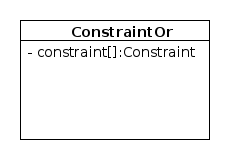
\includegraphics[scale=0.6]{./diagram_pictures/reactor/ConstraintOr.png}
		\caption{The ConstraintOr class}
	\end{minipage}
	\hfill
	\begin{minipage}[t]{8cm}
		\vspace{10pt}
			
	\end{minipage}
\end{figure}  

\subsubsection{Attributes}
\begin{itemize}
	\item \textbf{ private Constraint[] constraint }\\
	Contains constraints to be evaluated with an logical or.
\end{itemize}
\subsubsection{Methods}
\begin{itemize}
	\item \textbf{ public boolean evaluate\_constraint(RatedStatisticStorage) }\\
	Returns true if the evaluation of at least one constraint returns true.
\end{itemize}


\newpage
\subsection{ConstraintNot}
\begin{figure}[htbp]
	\begin{minipage}[t]{8cm}
		\vspace{0pt}
		\centering
		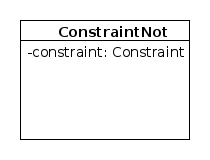
\includegraphics[scale=0.6]{./diagram_pictures/reactor/ConstraintNot.png}
		\caption{The ConstraintNot class}
	\end{minipage}
	\hfill
	\begin{minipage}[t]{8cm}
		\vspace{10pt}
			
	\end{minipage}
\end{figure}  

\subsubsection{Attributes}
\begin{itemize}
	\item \textbf{ private Constraint constraint }\\
	The constraint to be evaluated negated.
\end{itemize}
\subsubsection{Methods}
\begin{itemize}
	\item \textbf{ public boolean evaluate\_constraint(RatedStatisticStorage) }\\
	Returns true if the evaluation of the constraint returns false.
\end{itemize}


\newpage
\subsection{Enum Outcome}
\begin{figure}[htbp]
	\begin{minipage}[t]{8cm}
		\vspace{0pt}
		\centering
		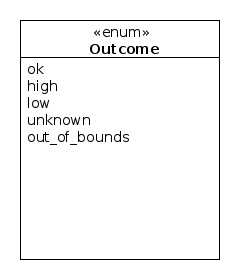
\includegraphics[scale=0.6]{./diagram_pictures/reactor/Outcome.png}
		\caption{The Outcome enum}
	\end{minipage}
	\hfill
	\begin{minipage}[t]{8cm}
		\vspace{10pt}
			
	\end{minipage}
\end{figure}  

\subsubsection{Types}
\begin{itemize}
	\item \textbf{ high }\\
	Data value is too high.
	\item \textbf{ low }\\
	Data value is too low.
	\item \textbf{ unknown }\\
	Data value is unknown.
	\item \textbf{ out\_of\_bounds }\\
	Data value is either too high or too low.
\end{itemize}


\newpage
\subsection{Reaction}
\begin{figure}[htbp]
	\begin{minipage}[t]{8cm}
		\vspace{0pt}
		\centering
		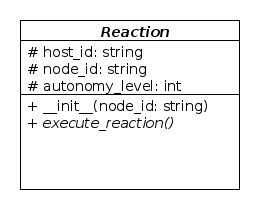
\includegraphics[scale=0.6]{./diagram_pictures/reactor/Reaction.png}
		\caption{The Reaction class}
	\end{minipage}
	\hfill
	\begin{minipage}[t]{8cm}
		\vspace{10pt}
			Abstract Reaction to an Constraint.
	\end{minipage}
\end{figure}  

\subsubsection{Attributes}
\begin{itemize}
	\item \textbf{ protected string host\_id }\\
		Contains the host on which the node is run on.
	\item \textbf{ protected string node\_id }\\
		The id of the node the reaction is ment to act upon.
	\item \textbf{ protected int autonomy\_level }\\
		This constraint only gets evaluatet if 
		the autonomy\_level is <= reaction\_autonomy\_level.
\end{itemize}
\subsubsection{Methods}
\begin{itemize}
	\item \textbf{ public void \_\_init\_\_(string node\_id) }\\
		Initializes the reaction. Sets the node to execute the reaction on. finds the corresponding host to the given node.
	\item \textbf{ public void execute\_reaction() }\\
		Executes the reaction as a service call to the HostStatistic node.
\end{itemize}

\newpage
\subsection{ReactionRun}
\begin{figure}[htbp]
	\begin{minipage}[t]{8cm}
		\vspace{0pt}
		\centering
		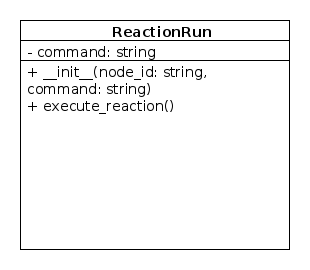
\includegraphics[scale=0.6]{./diagram_pictures/reactor/ReactionRun.png}
		\caption{The ReactionRun class}
	\end{minipage}
	\hfill
	\begin{minipage}[t]{8cm}
		\vspace{10pt}
			An Reaction which executes a command on the remote machine the specified node runs on. 
	\end{minipage}
\end{figure}

\subsubsection{Attributes}
\begin{itemize}
	\item \textbf{ private string command }\\
	Contains the command to be executed.
\end{itemize}
\subsubsection{Methods}
\begin{itemize}
	\item \textbf{ public void \_\_init\_\_(string node\_id,string command) }\\
		Initializes the reaction. Set the command to be executed.
	\item \textbf{ public void executeReaction() }\\
\end{itemize}


\newpage
\subsection{ReactionDefault}
\begin{figure}[htbp]
	\begin{minipage}[t]{8cm}
		\vspace{0pt}
		\centering
		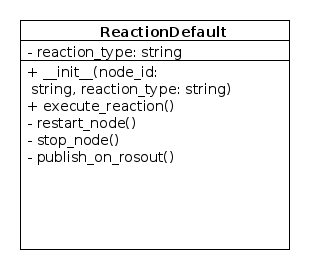
\includegraphics[scale=0.6]{./diagram_pictures/reactor/ReactionDefault.png}
		\caption{The ReactionDefault class}
	\end{minipage}
	\hfill
	\begin{minipage}[t]{8cm}
		\vspace{10pt}
			
	\end{minipage}
\end{figure}  

\subsubsection{attributes}
\begin{itemize}
	\item \textbf{ private ReactionDefaultType reaction\_type}\\
		Contains the type this reaction is of.
\end{itemize}
\subsubsection{Methods}
\begin{itemize}
	\item \textbf{ public void \_\_init\_\_(string node\_id, string reactionType) }\\
		Initializes the reaction. sets the reactiontype of this reaction.
	\item \textbf{ public void exececute\_reaction() }\\
	\item \textbf{ private void restart\_node() }\\
		Restarts the Node.
	\item \textbf{ private void stop\_node() }\\
		Stops the Node.
	\item \textbf{ private void publish\_on\_rosout() }\\
		Publishes the cause of the reaction on rosout.
\end{itemize}



\newpage
\subsection{Enum ReactionDefaultType}
\begin{figure}[htbp]
	\begin{minipage}[t]{8cm}
		\vspace{0pt}
		\centering
		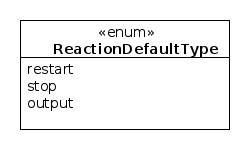
\includegraphics[scale=0.6]{./diagram_pictures/reactor/ReactionDefaultType.png}
		\caption{The ReactionDefaultType enum}
	\end{minipage}
	\hfill
	\begin{minipage}[t]{8cm}
		\vspace{10pt}
			
	\end{minipage}
\end{figure}  


\subsubsection{Types}
\begin{itemize}
	\item \textbf{ restart }\\
		Reaction is a restart of an entity.
	\item \textbf{ stop }\\
		Reaction is stopping an entity.
	\item \textbf{ output }\\
		Reaction is publishing the reaction on rosout.
\end{itemize}


\newpage
\subsection{HostLookUp}
\begin{figure}[htbp]
	\begin{minipage}[t]{8cm}
		\vspace{0pt}
		\centering
		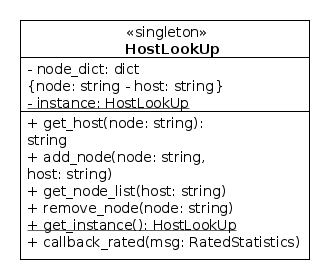
\includegraphics[scale=0.6]{./diagram_pictures/reactor/HostLookUp.png}
		\caption{The HostLookUp class}
	\end{minipage}
	\hfill
	\begin{minipage}[t]{8cm}
		\vspace{10pt}
			Singleton. Contains a dictionary of all nodes which are on an host who has an HostStatisticNode running and the hosts they run on.
	\end{minipage}
\end{figure}  


\subsubsection{Attributes}
\begin{itemize}
	\item \textbf{ private dict\{string node - string host\} node\_dict }\\
		Contains all nodes which are on an host who has an HostStatisticNode running. Host is the host the node runs on.
	\item \textbf{ private static HostLookUp instance }\\
		The singleton instance.
\end{itemize}
\subsubsection{Methods}
\begin{itemize}
	\item \textbf{ public string get\_host(string node) }\\
		Returns the host the node runs on.
	\item \textbf{ public void add\_node(string node, string host) }\\
		Adds an node - host tuple to the dictionary.
	\item \textbf{ public list<string> get\_node\_list(string host\_id) }\\
		Returns all nodes of a specifid host.
	\item \textbf{ public void remove\_node(string node) }\\
		Removes an node from the dictionary.
	\item \textbf{ public static HostLookUp get\_instance() }\\
		Returns the instance of HostLookUp.
	\item \textbf{ public void callback\_rated(RatedStatistics msg)}\\
		Callback for rated statistics. Adds unseen nodes to the dictionary.
\end{itemize}